\section{Blockchain for Local Governance Applications}

Blockchain is a technology that has been popular for its ability to have an immutable, transparent and decentralized ledger for public data. Hence, its a transformative tool for e-governance to address the problems that existing implementations had. The Blockchain allow us to verify the immutability of the records, so its suitable for governance applications where the trust and the accountability is crucial. \cite{hamill2018blockchain}, \cite{goswami2020egovernance}.

Blockchain based land registry system implemented in Cook Country, Illinois is a one real world example of the applicability of blockchain in local governance. They aim to reduce the property fraud by consolidating historical ownership records into a verifiable block in the blockchain. Similar to that Delaware has taken initiative to explore the use of smart contracts that's enable real time asset tracking and automate business fillings. This improves the regulatory compliance and oversights \cite{goswami2020egovernance}.

In addition to administrative efficiency, blockchain has been utilized for citizen centric services, such as secure digital identity management. Estonia has taken a initiative to integrate blockchain across healthcare, taxation and even electronic voting systems. So this can provide a mathematically verifiable audit trail for government data. MyPass project in Austin and the World Food Program's building blocks initiative also use Blockchain technology under the hood to manage encrypted identity and transaction records \cite{hamill2018blockchain}.

Despite the advancements in the blockchain base applications, existing literature highlights the challenges of adoption in governance. Scalability constraints, privacy concerns related to identity data, performance overhead and also the need of the legislative and institutional reforms are  some examples. These factors needs to be addressed by carefully selecting blockchain architectures and consensus mechanisms before implementing systems for frequent citizen interactions.

\section{Blockchain-Based Citizen Reporting and Complaint Management Systems}

The traditional centralized platforms have data integrity issues, transparency issues and trust issues when it comes to citizen reporting. Past works also indicates that centralized complaint registries often have single point of failures , delayed responses and public mistrust. Therefore blockchain integrated reporting services can be used to mitigate those issues. 

A blockchain based police complaint management system has proposed by Pratheeba \cite{pratheeba_blockchain_police_complaint} contains a modular architecture. It's include security, blockchain, web interface and a hybrid cloud storage. This system ensure immutability of complaint records by cryptographic hash linking. And also it utilize RSA based encryption to restrict the access only to authorized personnel. In Addition to that, Pratheeba used a Natural Language Processing (NLP) techniques to automatically categorize complaints in the system based on their priorities. 

\begin{figure}[h!]
    \centering
    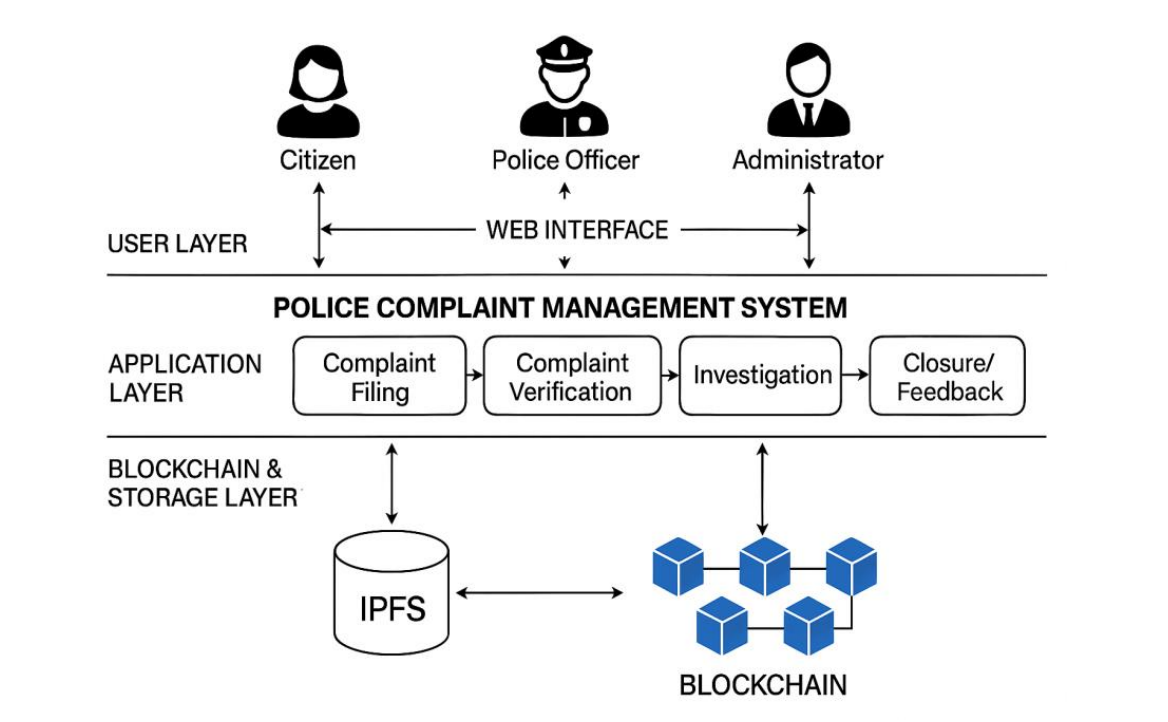
\includegraphics[width=0.95\textwidth]{figures/system-architecture-police-complaint-system.png} % Replace with your image file
    \caption{System Architecture of the Police Complaint Management System.\cite{manjula2025decentralized}}
    \label{fig:complaint-managment-system-architecture}
\end{figure}


A three tier architecture for decentralized complaint management framework has proposed by Manjula \cite{manjula2025decentralized} is shown in the Figure \ref{fig:complaint-managment-system-architecture}. The three layers are web based presentation layer, a business logic layer and finally a blockchain data layer. This system has a role based access control method to involve multiple stakeholders. Citizens, Law enforcement authorities and judicial bodies are some of them. More importantly this system has a immutable storage for multimedia evidences. Intelligent complaint assignment based on workloads, automatic escalation mechanism are some of the key features of the framework. The experimental evaluations shows that a significant reductions in complaint processing time. The successful detection of data tampering also archived by blockchain verification.

In literature, existing blockchain based complaint management systems shows some improvements in transparency and administrative efficiency. But most of them are domain specific. They primarily target law enforcement or isolated governance functions. In addition to that several platforms still rely on centralized architectures. Only a limited attention is given for implementing a community assisted validation, for privacy preserving reporting mechanisms and efficient handling of multimedia evidences. Therefore these limitations highlight the need for a generalized reporting framework for local governance.